80. $$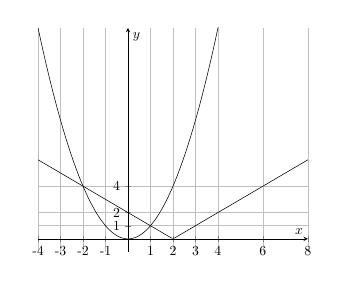
\begin{tikzpicture}[scale=0.5]
\begin{axis}[
    axis lines = middle,
    grid=major,
    legend pos={south west},
    xlabel = {$x$},
    ylabel = {$y$},
    ymin=-1,
    ymax=16,
    xtick={-3, -4, -1, 1, 4,3, 6,-2,2,8},
    xticklabels={-3, -4, -1, 1, 4,3, 6,-2,2,8},
    ytick={-14,-7,-2,1,2,4},
    yticklabels={-14,-7,-2,1,2,4}            ]
	\addplot[domain=-4:8, samples=100, color=black] {x*x};
\addplot[domain=-4:8, samples=100, color=black] {abs(x-2)};
%\addplot[domain=-3.1:2.5, samples=100, color=red] {70*abs(1-2*abs(abs(x)-2))-10*x^2+10*x-70};
	%\addlegendentry{$\text{Рис. 1}$};
\end{axis}
%\draw (0.85,2.35) circle (2pt);
\end{tikzpicture}$$
С осями эти графики пересекаются в точках $(0;0)$ и $(2;0),$ а между собой --- в точках $(-2;4)$ и $(1;1).$\\
